\documentclass[10pt, hyperref={unicode}]{beamer}

\usepackage[czech]{babel}
\usepackage[utf8]{inputenc}
\usepackage{times}
\usepackage{listings}
\usepackage{graphics}
\usepackage[ruled, czech, linesnumbered, noline, longend]{algorithm2e}

\mode<presentation> {
  \usetheme{Warsaw}
  \setbeamercovered{transparent}
}


\title{Grafové algoritmy - Depth-First Search}
\author{Daniel Štěpánek}
\institute[FIT VUT]{Fakulta informačních technologií VUT Brno}
\date{\today}

\begin{document}

\begin{frame}
	\titlepage
\end{frame}

\begin{frame}
	\frametitle{Osnova}
	\tableofcontents
\end{frame}


\section{Definice}
\begin{frame}
	\frametitle{Definice}
	\begin{itemize}
  		\item Grafový algoritmus pro procházení grafů metodou \emph{backtrackingu}.
  		\begin{block}{Backtracking}
			\begin{itemize}
				\item Způsob řešení algoritmických problémů založený na prohledávání stavového prostoru problému
				\item Problém osmi dam, jezdcova procházka
			\end{itemize}			    					
  		\end{block}
  		\item \emph{Vstup:} (ne)orientovaný graf
  		\item \emph{Výstup:} strom prohledávání do hloubky
	\end{itemize}
\end{frame}

\section{Základní typy grafů}
\begin{frame}
	\frametitle{Orientovaný vs. neorientovaný graf}
	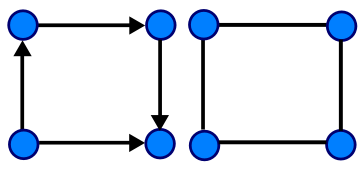
\includegraphics[scale=0.75]{img/or_vs_neor.png}
\end{frame}

\section{Ukázka kódu}
%http://www.mathcs.emory.edu/~cheung/Courses/171/Syllabus/11-Graph/dfs.html
\begin{frame}
	\begin{algorithm}[H]
	Set all nodes to "not visited"; \\
	s = new Stack(); \\
	s.push(initial node); \\
	\While{s $\neq$ empty}{
		x = s.pop(); \\
		\If{x has not been visited}{
			visited[x] = true; \\
			\For{every edge (x, y)}{
				\If{y has not been visited}{
				s.push(y);
				}			
			}
		}
	}
	\caption{Depth-First Search}
	\end{algorithm}
	\url{http://www.mathcs.emory.edu/~cheung/Courses/171/Syllabus/11-Graph/dfs.html}
\end{frame}

\section{Příklad}
\begin{frame}
	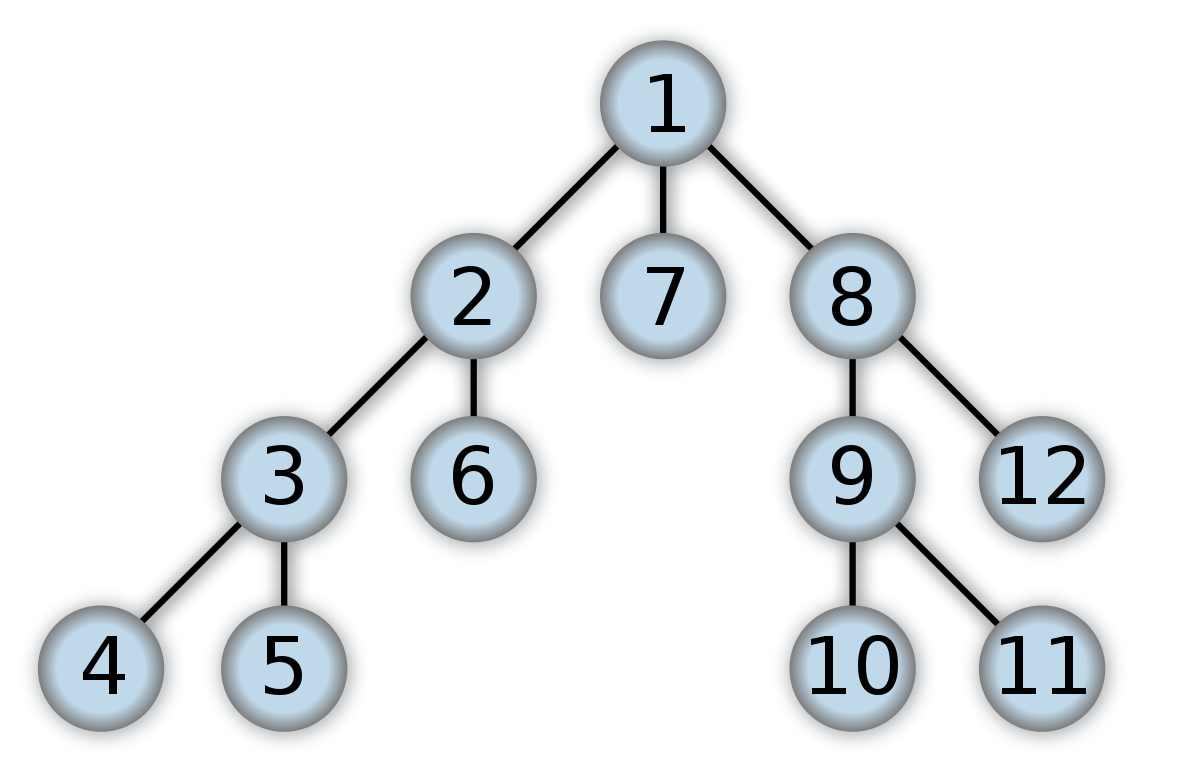
\includegraphics[scale=0.25]{img/dfs_tree.png}
\end{frame}

\section{Vlastnosti algoritmu}
\begin{frame}
	\frametitle{Vlastnosti algoritmu}
	\begin{block}{Úplnost}
			\begin{itemize}
				\item Na konečném grafu úplný
				\item Na nekonečném grafu neúplný
			\end{itemize}			    					
  		\end{block}
  	\begin{block}{Optimálnost}
			\begin{itemize}
				\item Stromová struktura: optimální
				\item Jiné struktury: není optimální
			\end{itemize}			    					
  		\end{block}
  	\begin{block}{Složitost}
  			Celková složitost algoritmu : $\Theta(|V| + |E|)$, kde:
			\begin{itemize}
			\item $|V|$ je počet vrcholů
			\item $|E|$ je počet hran daného grafu  	
			\end{itemize}				    					
  		\end{block}	 
\end{frame}

\begin{frame}
	\frametitle{Použité zdroje}
	\begin{itemize}
	\item \url{http://www.mathcs.emory.edu/~cheung/Courses/171/Syllabus/11-Graph/dfs.html}
	\item \url{https://en.wikipedia.org/wiki/Depth-first_search}
	\end{itemize}		
\end{frame}

\end{document}
